\section{Durchführung und Versuchsaufbau}

Damit die Kristallstruktur der zu untersuchenden Probe bestimmt werden kann, soll diese mit Röntgenstrahlung bestrahlt werden.
Es ist zu beachten, dass vor Beginn der Messung die Probe richtig präperiert wird. Dazu wird diese mit Hilfe eines Mörsers zerkleinert und anschließend in einen vorgefetteten
Zylinder gefüllt.
Dadurch sind die Ausrichtungen der Kristalline statistisch verteilt und es ist gewährleistet, dass Bragg-Reflexionen in allen Richtungen auftreten.
Anschließend kann die Probe im Versuchsaufbau platziert werden. Ein Elektromotor dreht die Probe während der Messung, damit auch bei grobkörnigen Probenmaterial
die Kristalline verteilt sind.\newline
Die Bragg-Reflexe sollen mit Hilfe eines Fotofilms detektiert werden. Aus diesem Grund wird ein Filmstreifen ringförmig um die Probe befestigt. Der Filmstreifen besitzt zwei Öfnnungen für den
Röntgenstrahl. Diese Öffnungen liegen so, dass der Röntgenstrahl sie ohne Reflexion durchläuft und sie makieren gleichzeitig die $180\,\text{°}$ Ebene.
Die Röntgenstrahlung wird durch eine Kupferanode erzeugt. Wenn diese auf die Probe trifft, wird sie mit dem Öffnungswinkel $2\theta$ gestreut. Das Beugungsmuster kann anschließend auf dem
Filmstreifen sichtbar gemacht werden.
Eine Darstellung des Versuchsaufbaus ist in Abbildung \ref{abb:aufbau} dargestellt.\newline
Die Messung wird für zwei verschiedene Proben durchgeführt. Um die Bragg-Reflexionen auf dem Film möglichst genau auswerten zu können, werden die Proben jeweils
$3\,\text{Stunden}$ lang bestrahlt.

\begin{figure}
  \centering
  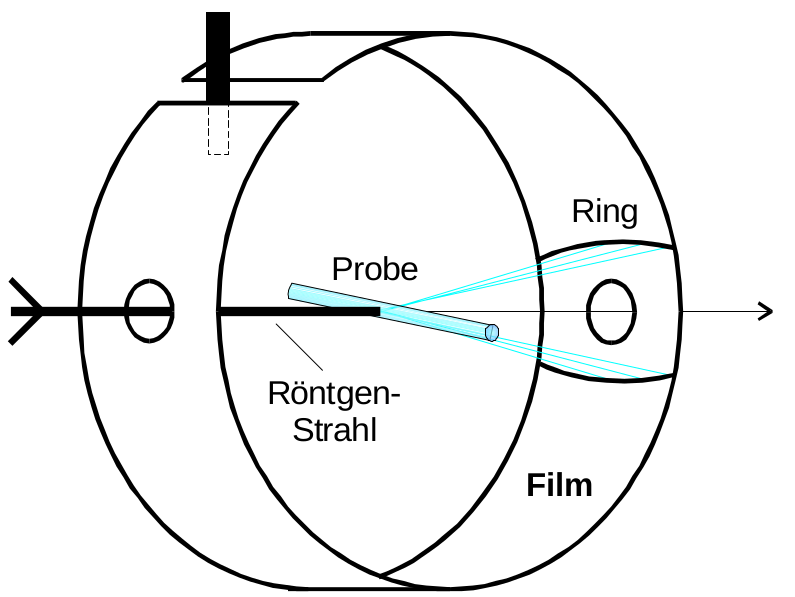
\includegraphics[scale=0.35]{aufbau.png}
  \caption{Versuchsaufbau zur Kristallstrukturbestimmung mit Hilfe des Debye-Scherrer-Verfahrens. In der Abbildung wird die Filmmethode dargestellt. Die Röntgenstrahlen werden an der zylindrischen
  Probe gebeugt. Das Beugungsmuster kann anschließend auf dem Filmstreifen sichtbar gemacht werden.}
  \label{abb:aufbau}
\end{figure}
